\Askhsh{14538}{2}
\begin{ylh}{1}
    \item 8.1. Όμοια ευθύγραμμα σχήματα
    \item 8.2. Κριτήρια ομοιότητας.
\end{ylh}
\begin{wrapfigure}[7]{r}{7.5cm}
    \centering
    \begin{tikzpicture}[scale=1]
        % Define Gamma as the origin
        \tkzDefPoint(0,0){G} % Gamma
        
        % Define points A and E such that A, Gamma, E are collinear and AG = 2GE
        % If E is at (x,y), then A is at (-2x, -2y)
        \tkzDefPoint(2.5,-1.25){E}
        \tkzDefPoint(-5,2.5){A}
        
        % Define points B and Delta such that B, Gamma, Delta are collinear
        % and AB || Delta E. From similarity, BG = 2GDelta
        % If B is at (x',y'), then Delta is at (-x'/2, -y'/2)
        \tkzDefPoint(-4,-2){B}
        \tkzDefPoint(2,1){D} % Delta
        
        % Draw the intersecting lines AΓΕ and ΒΓΔ
        \tkzDrawSegment[l3,maincolor](A,E)
        \tkzDrawSegment[l3,maincolor](B,D)
        
        % Draw the parallel segments AB and ΔE
        \tkzDrawSegment[l3,secondarycolor](A,B)
        \tkzDrawSegment[l3,secondarycolor](D,E)
        
        % Draw points
        \tkzDrawPoints(A,B,G,D,E)
        
        % Labels
        \tkzLabelPoint[above left](A){A}
        \tkzLabelPoint[below left](B){B}
        \tkzLabelPoint[below right](G){$\Gamma$}
        \tkzLabelPoint[above right](D){$\Delta$}
        \tkzLabelPoint[below right](E){E}
    \end{tikzpicture}
\end{wrapfigure}
Στο παρακάτω σχήμα τα τμήματα $\mathrm{AB}$ και $\mathrm{\Delta E}$ είναι παράλληλα και τα τμήματα $\mathrm{A\Gamma}$ και $\mathrm{\Gamma E}$ είναι τέτοια, ώστε $\mathrm{A\Gamma}=2\mathrm{\Gamma E}$.
\begin{alist}
\item Να αποδείξετε ότι τα τρίγωνα $\mathrm{AB\Gamma}$ και $\mathrm{E\Delta\Gamma}$ είναι όμοια. \monades{13}
\item
    \begin{rlist}
    \item Να γράψετε τους λόγους των ομόλογων πλευρών των δύο τριγώνων.
    \item Ποιος είναι ο λόγος ομοιότητας των δύο τριγώνων;
    \end{rlist} \monades{12}
\end{alist}